\documentclass{article}
\usepackage[utf8]{inputenc}
\usepackage{graphicx}

\title{IE 498 HW1}
\author{Yifan Shi(yifans16)}
\date{February 3, 2020}

\begin{document}

\maketitle

At first, I used sigmoid function as 
my activation function and set 150 units 
in the hidden layer. I also set the number 
of epoch to be 50000 and assigned a 
decreasing function for the learning rate 
$\alpha$ in order to update it in each epoch. 
 I initialized the weights $w$ and $c$ from 
 $Gaussian(0,0.1)$ and $Gaussian(0,0.2)$. 
 The bias $b^1$ and $b^2$ were both initialized 
 as zero vectors.


 In my for loop which performs the fully
 connected neural network, firstly I set an 
 index variable $i$ which is randomly picked 
 in each iteration and select $i^th$ row of
 my $train(x)$ array as the input layer. What's 
 following is just feed-forward and back 
 propagation steps which provides me better 
 parameters. 


However, when I applied the updated parameters 
onto my training and testing datasets, both of 
their prediction accuracy were only less than 70 
percent. Then I decided to use mini-batch, 
momentum in $SGD$ and to adjust the initial values
of the weights $w$ and $c$ as well as the learning 
rate $\alpha$.


The batch size I used was 150, so I also changed
the bias vectors $b^1$ and $b^2$ to be matrices 
with 150 columns and changed the index $i$ to be 
a 150-dimensional vector before the feed-forward 
step. Another new hyperparameter $\beta$ used in 
the momentum was set as 0.9 while the momentum, 
also updated for each epoch, can make the potential 
of the decrease on the weights become slightly 
larger. Lastly, I changed the initialization of 
the weights $w$ and $c$ to be $Gaussian(0,0.05)$ 
and $Gaussian(0,0.2)$, and make the learning rate
$/alpha$ to be constantly 0.0005. 


The accuracy I got when the final parameters 
applied to the training and testing datasets 
were 99.998 and 98.010 percent. (Figure\ 1)

\begin{figure}[h]
    \centering
    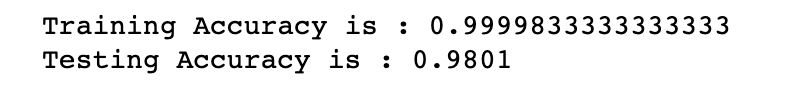
\includegraphics[scale=0.6]{accuracy.png}
  \end{figure}
\centering Figure\ 1: Prediction Accuracy.


\end{document}